% PROTOKOLL Action Item
\documentclass[
   draft=false
  ,paper=a4
  ,twoside=false
  ,fontsize=11pt
  ,headsepline
  ,DIV=11
  ,parskip=full+
  ,titlepage
]{scrartcl} % copied from Thesis Template from HAW

\usepackage[ngerman,english]{babel}

\usepackage[T1]{fontenc}
\usepackage[utf8]{inputenc}

\usepackage[
    left  =4em
   ,right =4em
   ,top   =5em
   ,bottom=5em
]{geometry}

\usepackage{longtable}
\usepackage[german,refpage]{nomencl}

\usepackage{float}
%\usepackage{enumitem}
\usepackage{paralist} %compactitem
\usepackage{graphicx}
%\usepackage{url}



\usepackage{hyperref} % for a better experience

\hypersetup{
   colorlinks=true % if false - links get colored frames
  ,linkcolor=black % color of tex intern links
  ,urlcolor=blue   % color of url links
  ,citecolor=black
}

\usepackage{amsmath}

\usepackage{array}   % for \newcolumntype macro
\newcolumntype{L}{>{$}l<{$}} % math-mode version of "l" column type
\newcolumntype{R}{>{$}r<{$}} % math-mode version of "r" column type
\newcolumntype{C}{>{$}c<{$}} % math-mode version of "c" column type

\usepackage{color}
\definecolor{black}{rgb}{0,0,0}
\definecolor{darkgray}{rgb}{0.2,0.2,0.2}
\definecolor{lightgray}{rgb}{0.9,0.9,0.9}
\definecolor{blue}{rgb}{0.0,0.0,0.9}
\definecolor{orange}{rgb}{0.7,0.3,0.0}
\definecolor{green}{rgb}{0.0,0.7,0.0}
\definecolor{red}{rgb}{0.9,0.0,0.0}

\usepackage{listings, lstautogobble}
\lstset{%
   language=bash
  ,frame=single
  ,numbers=left
  ,numberstyle=\tiny\color{darkgray}
  ,stepnumber=1
  ,numbersep=5pt
  ,backgroundcolor=\color{lightgray}
  ,showspaces=false
  ,keepspaces=true
  ,autogobble=true 
  ,breaklines=true
  ,tabsize=2
  , 
  ,basicstyle=\footnotesize\ttfamily\color{black}
  ,identifierstyle=\color{black}
  ,keywordstyle=[1]\color{blue}\textbf
  ,keywordstyle=[2]\color{red}\textbf
  ,stringstyle=\color{green}
  ,commentstyle=\color{darkgray}\textit
}
  
\usepackage{caption}
\usepackage{colortbl}
\definecolor{tabgrey}{rgb}{0.85,0.85,0.85}
%using minted because of the hashtag in bash

\sloppy
\clubpenalty=10000
\widowpenalty=10000
\displaywidowpenalty=10000


\usepackage{filecontents}

\usepackage{natbib}



% set font 
%\renewcommand{\familydefault}{\sfdefault}
\usepackage{times}

\begin{document}

\selectlanguage{ngerman}
% ----------------------------------------------------------------------------
% ---------------------------------------------------------- HIER WAS MACHEN -
% -------------------------------- Metadaten wie namen und Gruppentreffen etc-
\title{Aufgabenblatt 6: Schnelles Sortieren}
\subtitle{Praktikum: Algorithmen und Datenstrukturen für technische Informatiker}
\author{Martin Witte}
\author{%
        Martin Witte 
        \\ Karl-Fabian Witte
       }
\date{\today}

\publishers{%
	\normalfont\normalsize%
	\parbox{0.8\linewidth}{\centering
	  Der Algorithmus Quicksort wird für eine spezielle Keyverteilung
	  optimiert. Die Optimierung wird erklärt. Eine empirische Messung
	  wird quantitativ aufbereitet und das Ergebnis dargeboten.
	}
}

\maketitle
\setcounter{page}{1}
\tableofcontents
\flushleft

\section{Ausgangslage}
Quicksorts Aymptotische Komplexität liegt bei $O(n)=n\log(n)$ im \texttt{best}
und im \texttt{average case}. Im \texttt{worst case} ist die Komplexität bei 
$O(n)=n^2$. Dieser Fall liegt vor, wenn als Pivotelement immer ein Extrema
der zu sortierenden Liste ausgewählt wird und somit die Rekursionstiefe
wächst. 
Für kleine Listen ist Quicksort durch das \textbf{Teile und Herrsche Prinzip}
nicht geeignet, da es mehr konstanten Aufwand kostet, 
kleinere Listen zu unterteilen
und das Pivotelement mit höherer Wahrscheinlichkeit ein Extrema ist, sodass 
der \texttt{worst case} hier öfters eintreten kann. 
Zudem summieren sich die Konstanten Operationen (Pivotsuche und Swaping des
Pivots) auf, und bei einer Listengröße von $1$ ist dies ein Aufwand, der
keinen Nutzen hat.  

\section{Problemgrößen und Schlüsselverteilung}
Es soll eine Verbesserung des Quicksortalgorithmus gefunden werde, der die 
Anzahl der Operationen verkleinert. 

Die Elemente in den Listen, besitzen einen Schlüssel $k$, der 
aufsteigend sortiert wird. In Abhängigkeit der Anzahl der Elemente $N$, 
sind die Schlüssel wie folgt zu wählen:
\[
700N \leq k \leq 800N
\] 
Zudem sind die Schlüssel in diesem Wertebereich zufällig sortiert und es
können auch doppelte Schlüssel vorkommen.
Die Listengrößen 
\[
N = 10^i, i=1,2,\cdots,6
\]
werden hier untersucht.

\section{Verbesserungskonzept}

Um das unnötige Aufteilen von kleineren Listen zu verhindern, 
wird ab einer gewissen Mindestgröße der rekursive
Algorithmus (\textbf{Teile}) abgebrochen und durch einen anderen
Sortieralgorithmus, hier Insertionsort, ersetzt. \citep{ADskript}

Obwohl Insertionsort eine Komplexität von $O(n)=n^2$ hat, ist der Aufwand für 
kleine Problemgrößen $N$ meist geringer, 
da der konstante Faktor von Operationen im Quicksortverfahren hier entfällt. 

Die perfekte Abbruckgröße $S$ für die Quicksortrekursion ist nicht leicht zu
bestimmen, da diese von der Problemgröße und von der Sortiertheit der Liste 
anhängt. Es wurde daher keine Mathematische Formel für die Berechnung dieser
gefunden, sodass mehrere Abbruchgrößen empirisch verwendet werden. 

\section{Messung}

Es werden für die Messung folgende Größen betrachtet:
\begin{itemize}
  \item[moves] Bewegungsoperationen (Speicher wird neu belegt)
  \item[compares] Vergleichsoperationen (Vergleiche von Schlüsseln)
  \item[time] Die Zeit der Sortierung (Hardware abhängig)
\end{itemize}


Die Listen werden zufällig gefüllt. Das Quicksortverfahren sucht sich 
das Pivotelement zufällig aus der Teilliste. 
Um auswertbare Werte zu erhalten, werden alle Messungen $20$ mal wiederholt
und der Mittelwert gebildet. 
Als Abbruchsgröße für die Rekursion wird eine Listengröße von $N < S_i$ 
verwendet, wobei: 
\[
S_i= 10,20,\cdots,50
\]
ist.

Die Ergebnisse werden in doppellogarithmischen Diagrammen qualitativ und 
zudem in Tabellen quantitativ bewertbar dargestellt.

\begin{figure}[htp]
  \centering
  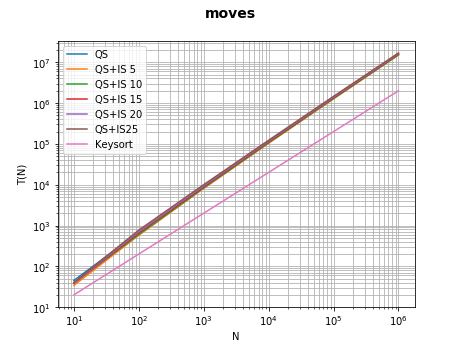
\includegraphics[width=\textwidth]{../moves.png}
  \caption[Bewegungen]{Darstellung der Anzahl der Zuweisungen der Listenenlemente $T(N)$ gegen die Problemgröße $N$}
  \label{fig:moves}
\end{figure}


\begin{table}[htp]
  \centering
  \caption[Bewegungen]{Die Anzahl der Zuweisungsbewegungen in Abhängigkeit 
  zur Listengröße $N$ der Implementationen ohne Insertion sort (normal) und
  mit Verschiedenen Abbruchbedingungsgrenzen (better$S$)}
  \label{tab:moves}
  \begin{tabular}{|r|r|r|r|r|r|r|r|}
  \hline
  $N$ & normal & better10 & better20 & better30 & better40 & better50 \\
  \hline
  10 & 47 & 39 & 40 & 39 & 40 & 40 \\
  100 & 684 & 607 & 601 & 608 & 599 & 602 \\
  1000 & 9184 & 8321 & 8318 & 8315 & 8349 & 8344 \\
  10000 & 114607 & 106208 & 106255 & 106291 & 106271 & 106116 \\
  100000 & 1374439 & 1291271 & 1294687 & 1291390 & 1291785 & 1294453 \\
  1000000 & 16028175 & 15228654 & 15229590 & 15205270 & 15234364 & 15217377 \\
  \hline
  \end{tabular}
\end{table}

In Abbildung \ref{fig:moves} ist nicht direkt etwas zu erkennen, jedoch sieht
man in Tabelle \ref{tab:moves} deutlich, dass der Insertionsort eine Verbesserung um ca. 1\% erbracht hat. Dabei unterschieden sich die Verfahren mit den unterschiedlichen Rekursionsabbruchkonstanten kaum von einander. 


\begin{figure}[htp]
  \centering
  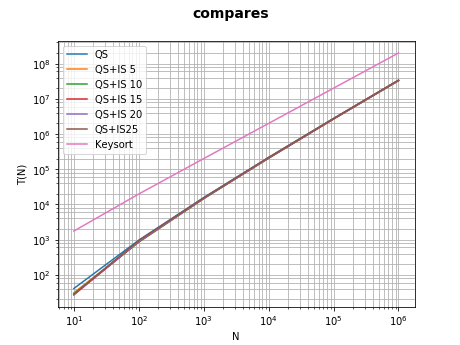
\includegraphics[width=\textwidth]{../compares.png}
  \caption[Vergleiche]{Darstellung der Anzahl der Schlüsselvergleiche 
  $T(N)$ gegen die Problemgröße $N$}
  \label{fig:compares}
\end{figure}

\begin{table}[htp]
  \centering
  \caption[Vergleiche]{Die Anzahl der Schlüsselvergleiche in Abhängigkeit 
  zur Listengröße $N$ der Implementationen ohne Insertion sort (normal) und
  mit Verschiedenen Abbruchbedingungsgrenzen (better$S$)}
  \label{tab:compare}
  \begin{tabular}{|c|r|r|r|r|r|r|r|}
  \hline
  $N$ & normal & better10 & better20 & better30 & better40 & better50 \\
  \hline
  10 & 40 & 28 & 29 & 29 & 29 & 29 \\
100 & 964 & 864 & 856 & 835 & 863 & 860 \\
1000 & 15534 & 14622 & 14600 & 14730 & 14488 & 14472 \\
10000 & 218299 & 207160 & 208889 & 206695 & 207246 & 208743 \\ 
100000 & 2784158 & 2694894 & 2675612 & 2694948 & 2687296 & 2683800 \\
1000000 & 34124652 & 32919852 & 32913209 & 33224115 & 32954215 & 32944586 \\
\hline
  \end{tabular}
\end{table}

Das selbe, wie in der Messung der Bewegungen, gilt auch hier. Abbildung \ref{fig:moves} und Tabelle \ref{tab:moves} weisen eine verbessung von ca. 1\% auf. 



\begin{figure}[htp]
  \centering
  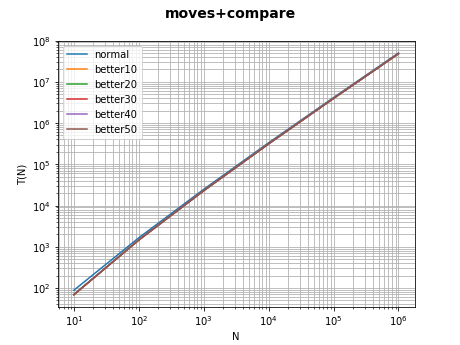
\includegraphics[width=\textwidth]{../moves+compare.png}
  \caption[Bewegungen und Vergleiche]{Darstellung der Schlüsselvergleiche und Zuweisungen zusammen $T(N)$ die Problemgröße $N$}
  \label{fig:total}
\end{figure}


\begin{table}[htp]
  \centering
  \caption[Bewegungen und Vergleiche]{Die Anzahl der Schlüsselvergleiche und Bewegungen in Abhängigkeit 
  zur Listengröße $N$ der Implementationen ohne Insertion sort (normal) und
  mit Verschiedenen Abbruchbedingungsgrenzen (better$S$)}
  \label{tab:total}
  \begin{tabular}{|c|r|r|r|r|r|r|r|}
  \hline
  $N$ & normal & better10 & better20 & better30 & better40 & better50 \\
  \hline
  10 & 88 & 68 & 69 & 69 & 69 & 69 \\
100 & 1649 & 1471 & 1457 & 1444 & 1462 & 1463 \\
1000 & 24718 & 22944 & 22919 & 23045 & 22838 & 22817 \\
10000 & 332906 & 313368 & 315145 & 312986 & 313518 & 314860 \\
100000 & 4158598 & 3986166 & 3970299 & 3986338 & 3979082 & 3978254 \\
1000000 & 50152827 & 48148506 & 48142799 & 48429385 & 48188579 & 48161963 \\
\hline
  \end{tabular}
\end{table}

Die Summe aus Bewegungen und Vergleichen liegt somit im selben Verhältnis, wie man Abbildung \ref{fig:total} und \ref{tab:total} vernehmen kann. 


\begin{figure}[htp]
  \centering
  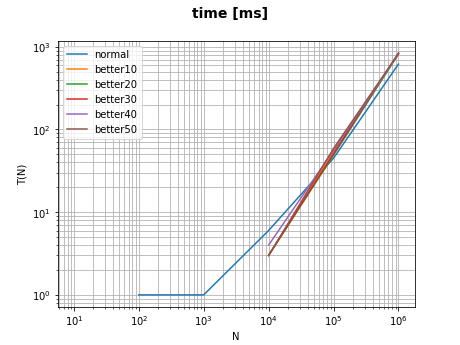
\includegraphics[width=\textwidth]{../time_ms.png}
  \caption[Zeit]{Darstellung benötigten Berechnungszeit $T(N)$ in
   Millisekunden gegen die Problemgröße $N$}
  \label{fig:time}
\end{figure}

\begin{table}[htp]
  \centering
  \caption[Bewegungen]{Die Berechnungszeit in $ms$ in Abhängigkeit 
  zur Listengröße $N$ der Implementationen ohne Insertion sort (normal) und
  mit Verschiedenen Abbruchbedingungsgrenzen (better$S$)}
  \label{tab:time}
  \begin{tabular}{|c|r|r|r|r|r|r|r|}
  \hline
  $N$ & normal & better10 & better20 & better30 & better40 & better50 \\
  \hline
  10 & 0 & 0 & 0 & 0 & 0 & 0 \\
100 & 1 & 0 & 0 & 0 & 0 & 0 \\
1000 & 1 & 0 & 0 & 0 & 0 & 0 \\
10000 & 6 & 3 & 3 & 3 & 4 & 3 \\
100000 & 45 & 54 & 49 & 51 & 56 & 59 \\
1000000 & 617 & 818 & 819 & 841 & 821 & 828 \\
\hline
  \end{tabular}
\end{table}

Die Zeitmessung weißt hingegen ein auffälligeres Verhalten auf. Abbildung \ref{fig:time} und Tabelle \ref{tab:time} zeigen, dass die weniger Aufwändige Variante des Quicksorts mit Insertion sort ab $N = 100.000$ deutlich mehr Rechenzeit benötigt. Da die Rekursion ständig den Stack belastet, hätte den 
reinen Quicksort mehr Zeit beansprucht, doch hier verhält sich der verbesserte
Algorithmus langsamer. Es wird vermutet, dass die Hardware bzw. die übersetzung der Virtuellen Maschine Javas die Rekursion gut optimiert.

\section{Ergebnis}

Eine Verbesserung mit dem Abbruch des rekursiven Verfahrens und der Sortierung der kleinen Teillisten mit Insertionsort ist nicht stark ausgefallen. Lediglich die Operationsanzahl hat sich um 1\% verbessert. 
Das die Laufzeit sich erhöht, ist nicht mit der Implementation zu erklären.

\begin{filecontents}{doc.bib}
@book{ADskript
  ,author    = {Pareigis, Stephan}
  ,title     = {Algorithmen und Datenstrukturen für Technische Informatiker}
  ,year      = {2017}
  ,publisher = {Hochschule für Angewanste Wissenschaften Hamburg}
  ,address   = {Department für Informatik}
}
\end{filecontents}
	
	
\bibliographystyle{plainnat}
\bibliography{git.bib}
\end{document}